\documentclass[12pt]{article}

\usepackage{epsfig}
\usepackage{pgf,tikz}
\renewcommand{\theenumi}{(\alph{enumi})} 
\renewcommand{\labelenumi}{\theenumi}

\pagestyle{empty}
\setlength{\textwidth}{7in}
\setlength{\oddsidemargin}{-0.5in}
\setlength{\topmargin}{-1.0in}
\setlength{\textheight}{9.5in}

\newtheorem{problem}{Problem}

\begin{document}

\noindent{\large\bf MA261}\hfill{\large\bf Exam\#1.}\hfill{\large\bf
  Spring 2007}\hfill{\large\bf Page 1/6}\hrule

\bigskip
\begin{center}
  \begin{tabular}{|ll|}
    \hline & \cr
    {\bf Name: } & \makebox[12cm]{\hrulefill}\cr & \cr
    {\bf 10-Digit PUID:} & \makebox[12cm]{\hrulefill}\cr & \cr
    {\bf Recitation Instructor:} & \hrulefill \cr & \cr
    {\bf Recitation Time:} & \hrulefill \cr & \cr
    \hline
  \end{tabular}
\end{center}
\begin{itemize}
\item Write your name, 10-digit PUID, recitation instructor's name and
  recitation time in the space provided above.
\item The test has six (6) pages, including this one.
\item For muli-choice questions, you should circle the answer you
  select.  On the other problems, you should enter your answer in the
  box(es) provided.
\item You must show sufficient work to justify all answers unless
  otherwise stated in the problem.  Correct answers with inconsistent
  work may not be given credit.
\item Credit for each problem is given in parentheses at the right of
  the problem nomber.
\item No books, notes or calculators may be used on this test.
\item Te solutions will be posted on the web in a few days:
  \texttt{www.math.purdue.edu/MA261}.
\end{itemize}
\hrule

\begin{center}
  \begin{tabular}{|c|c|c|}
    \hline
    &&\cr
    {\large\bf Page} & {\large\bf Max.~points} & {\large\bf Your points} \cr
    &&\cr
    \hline
    &&\cr
    {\Large 2} & \Large 10 & \cr
    &&\cr
    \hline
    &&\cr
    {\Large 3} & \Large 28 & \cr
    &&\cr
    \hline
    &&\cr
    {\Large 4} & \Large 30 & \cr
    &&\cr
    \hline
    &&\cr
    {\Large 5} & \Large 20 & \cr
    &&\cr
    \hline
    &&\cr
    {\Large 6} & \Large 12 & \cr
    &&\cr
    \hline\hline
    &&\cr
    {\large\bf Total} & \Large 100 & \cr
    &&\cr
    \hline
  \end{tabular}
\end{center}
\newpage

%%%%%%%%%%%%%%%%%%%%%%%%%%%%%%%%%%%%% Page 1
\noindent{\large\bf MA261}\hfill{\large\bf Exam\#1.}\hfill{\large\bf
  Spring 2007}\hfill{\large\bf Page 2/6}\hrule

\bigskip
{\problem[10 pts] \em Let $P(x,y,z)$, $Q(x-x,-y,-z)$ be two antipodal
  (opposite) points on $x^2+y^2+z^2=1$ and let $R(X,y,z)$ be any other
  point with $x^2+y^2+z^2=1$.  Then the angle between
  $\overrightarrow{PR}$ and $\overrightarrow{QR}$
  is}
\begin{enumerate}
\item $\pi/3$
\item $\pi/4$
\item $\pi/2$
\item $2\pi/3$
\item $\pi/6$
\end{enumerate}
\newpage

%%%%%%%%%%%%%%%%%%%%%%%%%%%%%%%%%%%%% Page 2
\noindent{\large\bf MA261}\hfill{\large\bf Exam\#1.}\hfill{\large\bf
  Spring 2007}\hfill{\large\bf Page 3/6}\hrule

\bigskip
{\problem[8pts] \em Find $x$ so that the vectors $(2,x,3)$ and
  $(-4,1,x)$ are orthogonal. $x=$}
\begin{enumerate}
\item $1/2$
\item $-1/2$
\item $2$
\item $0$
\item $1$
\end{enumerate}
\vspace{2cm}
\hrule

{\problem[10 pts] \em Let $P$ be the plane which contains the vectors
  $R(2,5,7)$, $S(-1,6,0)$ and $T(2,0,2)$.  The line through $P$ which
  contains the vector $R$ is}
\begin{enumerate}
\item $\displaystyle{\frac{x-2}{3} = \frac{y-5}{-6} = \frac{z-7}{-2}}$
\item $\displaystyle{\frac{x-2}{8} = \frac{y-5}{-3} = \frac{z-7}{-3}}$
\item $\displaystyle{\frac{x-2}{-8} = \frac{y-5}{-3} = \frac{z-7}{-8}}$
\item $\displaystyle{\frac{x-2}{8} = \frac{y-5}{3} = \frac{z-7}{-3}}$
\end{enumerate}
\vspace{2cm}
\hrule

{\problem[10 pts] \em The equation $x+1 = y^2+9z^2$ has a graph most like}
 \begin{center}
   \begin{tikzpicture}
     \shade (0cm,0cm) rectangle (\linewidth, 7cm);
     \draw (0.1\linewidth,0.5cm) node[rounded corners]{(a)};
     \draw (0.3\linewidth,0.5cm) node[rounded corners]{(b)};
     \draw (0.5\linewidth,0.5cm) node[rounded corners]{(c)};
     \draw (0.7\linewidth,0.5cm) node[rounded corners]{(d)};
     \draw (0.9\linewidth,0.5cm) node[rounded corners]{(e)};
   \end{tikzpicture}
 \end{center}
\newpage

%%%%%%%%%%%%%%%%%%%%%%%%%%%%%%%%%%%%% Page 3
\noindent{\large\bf MA261}\hfill{\large\bf Exam\#1.}\hfill{\large\bf
  Spring 2007}\hfill{\large\bf Page 4/6}\hrule

\bigskip
{\problem[10 pts] \em If $h(x,y) = \sin \Big( \displaystyle{\frac{x}{y^2}} \Big)$, then
$\displaystyle{\frac{\partial^2 h}{\partial x \partial y}}=$}
\begin{enumerate}
\item $\displaystyle{\frac{2x}{y^5} \sin\Big( \frac{x}{y^2} \Big) + \frac{2}{y^2} \cos \Big( \frac{x}{y^2} \Big)}$
\item $\displaystyle{\frac{2x}{y^5} \sin\Big( \frac{x}{y^2} \Big) - \frac{2}{y^3} \cos \Big( \frac{x}{y^2} \Big)}$
\item $-\displaystyle{\frac{1}{y^2} \sin\Big( \frac{x}{y^2} \Big) - \frac{2}{y^3} \cos \Big( \frac{x}{y^2} \Big)}$
\item $\displaystyle{\frac{x}{y^5} \sin\Big( \frac{x}{y^2} \Big) - \frac{1}{y^3} \cos \Big( \frac{x}{y^2} \Big)}$
\item $\displaystyle{\frac{2x}{y^5} \sin\Big( \frac{x}{y^2} \Big) - \frac{1}{y^3} \cos \Big( \frac{x}{y^2} \Big)}$
\end{enumerate}
\hrule

{\problem[10 pts] \em If $f(x,y) = xe^{2x+y}$, then }
$$ \lim_{h \to 0} \frac{f(1+h,0)- f(1,0)}{h} = $$
\begin{enumerate}
\item $e^2$
\item $-e^2$
\item $2e^2$
\item $3e^2$
\item $-2e^2$
\end{enumerate}
\vspace{2cm}
\hrule

{\problem[10 pts] \em The level curve $f=5$ of the function $f(x,y) =
  \displaystyle{ \frac{x^2+1}{x-y^2} }$ is}
\begin{enumerate}
\item an ellipse
\item a circle
\item a hyperbola
\item a parabola
\item a straight line
\end{enumerate}

\newpage

%%%%%%%%%%%%%%%%%%%%%%%%%%%%%%%%%%%%% Page 4
\noindent{\large\bf MA261}\hfill{\large\bf Exam\#1.}\hfill{\large\bf
  Spring 2007}\hfill{\large\bf Page 5/6}\hrule

\bigskip
{\problem[10 pts] \em The equation whose graph is the indicated figure
is}
\begin{enumerate}
\item $2x^2 + z^2 = -y$
\item $2x^2 + z^2 = y$
\item $2x^2 + z^2 = y^2+1$
\item $2x^2 + z^2 = y^2-1$
\item $2x^2 + z^2 = y-1$
\end{enumerate}
\vspace{2cm}
\hrule

{\problem[10 pts] \em Let $\mathbf{r}(t) = \big( x(t), y(t)
  \big)$, $t\geq 0$ denote the position of a particle at time $t$ with
  acceleration $\mathbf{a}(t) = (3t,-2)$, initial velocity
  $\mathbf{v}_0 = (2,5)$ and initial position $\mathbf{r}_0 =
  (0,50)$.  The value of $x(t)$ when $y(t)=0$ is}
\vspace{12cm}
\begin{flushright}
  \begin{tikzpicture}
    \draw (-1cm,0.5cm) node {$x(t) =$};
    \draw (0cm,0cm) rectangle (5cm,1.2cm);
  \end{tikzpicture}
%   $x(t)=$ \framebox[5cm]{\raisebox{1cm}[0.6cm][0.4cm]}
\end{flushright}
\newpage

%%%%%%%%%%%%%%%%%%%%%%%%%%%%%%%%%%%%% Page 5
\noindent{\large\bf MA261}\hfill{\large\bf Exam\#1.}\hfill{\large\bf
  Spring 2007}\hfill{\large\bf Page 6/6}\hrule

\bigskip
{\problem[12 pts] \em Find the equation of the tangent plane to the
  surface $z=5-2x^2-y^2$ at $(1,1,2)$, and the parametric equation of
  the perpendicular line to that plane at that point.}
\vspace{16cm}
\begin{flushright}
  \begin{tikzpicture}
    \draw(2.5cm,4.2cm) node {Tangent Plane:};
    \draw(5cm,3.7cm) rectangle (10cm,4.8cm);
    \draw(2.5cm,1.8cm) node {Perpendicular Line:};
    \draw(5cm,0cm) rectangle (10cm,3.6cm);
    \draw(5.5cm,3cm) node {$x=$};
    \draw(5.5cm,1.8cm) node {$y=$};
    \draw(5.5cm,0.6cm) node {$z=$};
  \end{tikzpicture}
%   Tangent Plane: \framebox[5cm]{\raisebox{1cm}[0.6cm][0.4cm]} \\
%   Perpendicular Line: \framebox[5cm]{\raisebox{1cm}[0.6cm][3.4cm]}
\end{flushright}
\end{document}
